\documentclass[12pt]{book}
\usepackage{graphicx}
\usepackage{subfig} % make it possible to include more than one captioned figure/table in a single float
\usepackage[utf8]{inputenc}
\usepackage{hyperref}
\usepackage[intlimits]{amsmath}
\usepackage{amssymb}
\usepackage{tkz-euclide}
\usepackage{tikz}
\setlength{\oddsidemargin}{15.5pt} 
\setlength{\evensidemargin}{15.5pt}
\pretolerance=2000
\tolerance=3000
\renewcommand{\figurename}{Figura}
\renewcommand{\chaptername}{Cap\'{i}tulo}
\renewcommand{\contentsname}{\'{I}ndice}
\renewcommand{\tablename}{Tabla}
\renewcommand{\bibname}{Bibliograf\'{i}a}
\renewcommand{\appendixname}{Ap\'endices}


\title{Sistema autogravitante con simetría esférica y distribución exponencial de masa}
\date{}
\begin{document}
\section*{Nociones teóricas}


\begin{footnotesize}
Notaciones: 
$\vec{x} = (x_1, x_2, x_3)$ para mostrar que $x = (x_1, x_2, x_3)$ es un vector $\in \mathbb{R}^3$
Para una function  $f \colon \mathbb{R}^3 \to \mathbb{R}^3$ $\vec{f}(\vec{x}) = (f_1(\vec{x}), f_2(\vec{x}), f_3(\vec{x}) )$ (vector)
y una  funcion $g \colon \mathbb{R}^3 \to \mathbb{R}$ (scalar)
\begin{description}
\item
$\nabla g(\vec{x}) = (\frac{\partial g}{\partial x_1}(\vec{x}), \frac{\partial g}{\partial x_2}(\vec{x}), \frac{\partial g}{\partial x_3}(\vec{x}) )$ es un  vector $\in   \mathbb{R}^3$;
\item
$\nabla  \cdot  \vec{f}(\vec{x}) =  \frac{\partial f_1}{\partial x_1}(\vec{x})+ \frac{\partial f_2}{\partial x_2}(\vec{x})+ \frac{\partial f_3}{\partial x_3}(\vec{x})$ es un scalar $(\in \mathbb{R})$
\item
$\nabla^2 g(\vec{x}) = \nabla  \cdot \nabla g(\vec{x}) = \frac{\partial^2 g}{\partial^2 x_1}(\vec{x})+ \frac{\partial^2 g}{\partial^2 x_2}(\vec{x})+ \frac{\partial^2 g}{\partial^2 x_3}(\vec{x})$ scalar $(\in \mathbb{R})
$
\end{description}
\end{footnotesize}


\begin{description}
\item Para una distribución de densidad de masa $\rho \colon \mathbb{R}^3 \to \mathbb{R}$
\item De la ley de Newton la fuerza gravitatoria ejercitada en una masa m = 1 situada en el punto x es:  $\vec{F}(\vec{x}) = G \int{\frac{\vec{x\prime} - \vec{x}}{|\vec{x\prime} - \vec{x}|^3}\rho(\vec{x\prime})d^3\vec{x\prime}} $ 
y despues de hacer cálculos llegamos a $ \nabla  \cdot  \vec{F}(\vec{x}) = -4\pi G \rho(\vec{x}) $
\item Definimos el potencial gravitatorio $\Phi(\vec{x}) = -G \int{\frac{\rho(\vec{x\prime})}{|\vec{x\prime} - \vec{x}|}d^3\vec{x}} $. 
Observamos que $\vec{F}(\vec{x}) = - \nabla \Phi(\vec{x}) $ 
y después de reemplazar en la ecuación de antes se obtiene la ecuación de Poisson: $\nabla^2 \Phi(\vec{x}) = 4\pi G \rho(\vec{x}) $
\item \textbf{En coordenadas esféricas} ($r,\theta,\varphi$) \textbf{con simetria esférica} 
(las funciones solo dependen de r ($=|\vec{r}|$) y no de la posición en la esfera de radio r: los angulos $\theta$ y $\varphi$ )

Las derivadas totales coinciden con las derivadas parciales $\frac {d\Phi(r)}{dr} = \frac{\partial \Phi(r)}{\partial r} $; 
$|\vec{F}(r)| = |\nabla \Phi(r)| = \frac{\partial \Phi(r)}{\partial r} $ y 
$\nabla^2 \Phi(r) = \frac{1}{r^2} \frac{\partial }{\partial r}(r^2 \frac{\partial \phi(r)}{\partial r})$
\item
La ecuacion Poisson:$ \frac{1}{r^2} \frac{\partial }{\partial r}(r^2 \frac{\partial \phi(r)}{\partial r}) = 4\pi G \rho(r) \implies
r^2 \frac{\partial \phi(r)}{\partial r} = 4\pi G \int{r^2\rho(r)dr} + K_1 \implies
\frac{\partial \Phi(r)}{\partial r} = \frac{4 \pi G}{r^2}\int{r^2\rho(r)dr} + \frac{K_1}{r^2}\implies
\Phi(r) = 4\pi G \int{\frac{1}{r^2}(\int{r^2\rho(r)dr})dr } + K_1\int{\frac{1}{r^2}dr} + K_2
=4\pi G \int{\frac{1}{r^2}(\int{r^2\rho(r)dr})dr } + \frac{K_1}{r} + K_2, K_1, K_2 \in \mathbb{R} (el signo - con K_1)
 $
\item El módulo de la fuerza ejercitada sobre la particula debido al movimiento en una órbita circular es $ |\vec{F}(r)| = m \frac{v_c^2}{r} $ y tiene que ser igual al  módulo la fuerza gravitatoria $\frac{\partial \Phi(r)}{\partial r}$
donde $v_c$ es el módulo de la velocidad circular y m se consideró = 1
$ \implies v_c^2(r) = r\frac{\partial \Phi(r)}{\partial r} \implies
v_c^2(r) = \frac{4\pi G}{r}\int{r^2\rho(r)dr} + \frac{K}{r}, K \in \mathbb{R} \implies 
v_c(r) = (\frac{4 \pi G}{r}\int{r^2\rho(r)dr} + \frac{K}{r})^{\frac{1}{2}}, K \in \mathbb{R}
$
\item La masa $M(r) = 4 \pi \int{r^2\rho(r)dr} + K, K \in \mathbb{R}$
\item Las constantes de integración se eligen de tal forma que verifiquen las condiciones de contorno:
 $\lim_{x \to +\infty}\Phi(x) = 0, v_c(0) = 0, M(0) = 0$

\item En un sistema con simetria esférica: la proyección de una función f(r) en el plano y,z (a lo largo de la línea de visión OX)es la funcción: 
$F(s) = \int_{-\infty}^\infty{f(r)dx}$ donde s es la distancia desde el centro del circulo en el plano proyectado ($s^2 = y^2 + z^2$)
\item $r^2 = x^2 + s^2$ y la simetría esférica $ \implies  F(s) =  2\lvert \int_0^\infty{f(\sqrt{x^2+s^2})dx} \rvert  $

\begin{tikzpicture}[scale=.8]

% definitions
\tkzDefPoint(0,0){O}
\tkzDefPoint(2,2){P}
\tkzDefPoint(0,2){M}
\tkzDefPoint(3.5,0){Q}
\tkzDefPoint(2.87,2){S}
\tkzDefPoint(-2.87,2){T}


\tkzDrawCircle(O,Q)
\draw [shorten >= -5cm, shorten <=-5cm] (S)--(T) ;
\tkzDrawSegments[thick](O,M)
\tkzDrawSegments[thick](O,P)
\tkzDrawPoints(O,P,Q,T,M,S)

\node at (6,2.2){line of sight};
\node at (-0.5,1){s};
\node at (0.7,0.5){r};
\node at (0.5,2.2){x};
% labels
\tkzLabelPoints(Q,T,O,M,S,P)
\end{tikzpicture}

\item Para calcular estas funciones de forma numérica hay que establecer los límites de integración y las constantes
\item Miramos los gráficos de las funciones que se integran:

\item $ f(r) = r^2 \rho(r)$
\item $g(r) = \frac{1}{r^2}  \int_0^r{\frac{1}{x^2} \rho(x) dx }$
\item si  f es  continua y f(0) = 0 y g no está definida en 0 pero es continua en (0,$\infty$) y $  \lim_{x \underset{>}{\to} 0} g(x) = 0$
\item $\Phi(r) = 4 \pi G  \int_\varepsilon^r{ \frac{1}{x^2}(\int_0^x{a^2 \rho(a)da})dx} + K_2$
(elegimos $K_1 = 0$ y $K_2$  de tal manera que $\lim_{x \to +\infty}\Phi(x) = 0 $, en práctica $K_2 = -\Phi(R_{max})$  y $\varepsilon \approx 0$ ) 
\item $v_c(r) = (\frac{4 \pi G }{r}\int_0^r{x^2 \rho(x)dx} )^{\frac{1}{2}}  $ (la constante de integración es 0 porque $v_c(0) = 0$)
\item $M(r) = 4 \pi \int_0^r{x^2 \rho(x)dx}$ (la constante de integración es 0 porque $M(0) = 0$) 
\end{description}

\section*{Problema de la práctica. Solución numérica}
\begin{description}
\item Hipótesis: $\rho(r) = \rho_c e^{-\frac{r}{r_0}} $
\item Determinar $\Phi(r)$, M(r),$M_p(r)$, $v_c(r)$ 

\end{description}


\begin{description}
\item Miramos los gráficos de las funciones f y g de arriba (plotFunctions.py) para poner los límites y constantes de integración en las funciones con las integrales calculadas de forma numérica(ver exp\_num.py)
\begin{figure}[!ht]
 \centering
 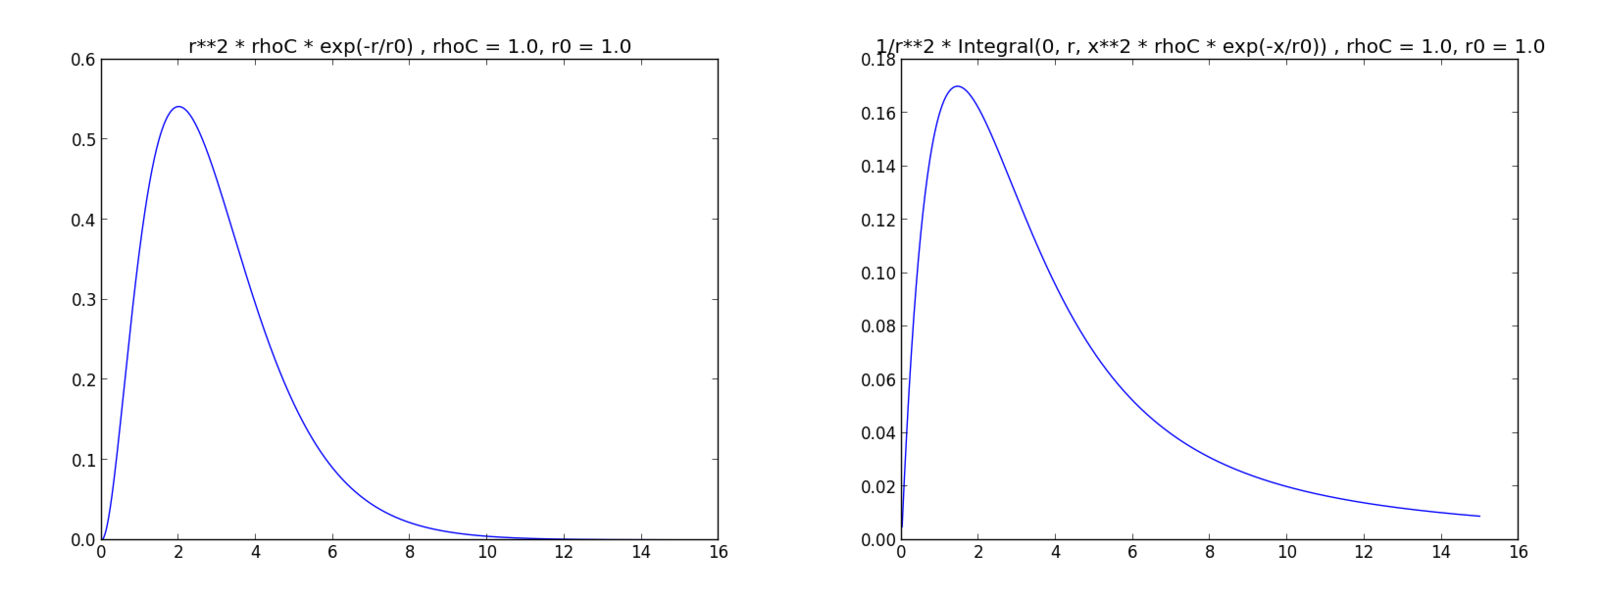
\includegraphics[scale=0.33]{func12Plot.png}
 \caption{\emph{Graficos de las funciones f y g}}
\end{figure}

\item $\Phi(r) = 4 \pi G \rho_c \int_\varepsilon^r{ \frac{1}{x^2}(\int_0^x{a^2 e^{-\frac{a}{r_0}}da})dx} -\Phi(R_{max})$
\item $v_c(r) = (\frac{4 \pi G \rho_c}{r}\int_0^r{x^2 e^{-\frac{x}{r_0}}dx} )^{\frac{1}{2}}  $ 
\item $M(r) = 4 \pi \rho_c \int_0^r{x^2 e^{-\frac{x}{r_0}}dx}$ 
\item La proyección de la distribución de densidad en el plano YOZ
$D_p(s) = 2 \rho_c \lvert \int_0^\infty{e^{-\frac{\sqrt{s^2 + x^2}}{r_0}} dx}  \rvert$


\end{description}





\section*{Solución analítica}
\begin{description}
\item Las integrales se pueden calcular de forma analítica, así que las funciones del potencial, masa y vc se pueden expresar sin usar integrales (ver exp\_an.py).

\item  $\rho(r) =  \rho_c  e^{-\frac{r}{r_0}} $  
\item Integrando por partes 2 veces:
\item $\int_0^r{x^2 e^{-\frac{x}{r_0}}dx} = - r_0 \int_0^r{x^2 (e^{-\frac{x}{r_0}})\prime dx}
=-r_0( (x^2 e^{-\frac{x}{r_0}})\Big|_0^r  - 2\int_0^r{x e^{-\frac{x}{r_0}}dx})  = 
-2 r_0^2 \int_0^r{x (e^{-\frac{x}{r_0}})\prime dx} - r_0 r^2 e^{-\frac{r}{r_0}} = -2 r_0^2 ((x e^{-\frac{x}{r_0}})\Big|_0^r - \int_0^r{e^{-\frac{x}{r_0}}dx}) - r_0 r^2 e^{-\frac{r}{r_0}} = 
-2 r_0^3 e^{-\frac{x}{r_0}}\Big|_0^r -2 r_0^2 r e^{-\frac{r}{r_0}} - r_0 r^2 e^{-\frac{r}{r_0}} = 
2 r_0^3 -2 r_0^3 e^{-\frac{r}{r_0}} -2 r_0^2 r e^{-\frac{r}{r_0}} - r_0 r^2 e^{-\frac{r}{r_0}}  
= 2  r_0^3 -  r_0 e^{-\frac{r}{r_0}} (2 r_0^2  + 2 r_0 r + r^2)
$

\item $\implies \int_\varepsilon^r{ \frac{1}{x^2}(\int_0^x{y^2 e^{-\frac{y}{r_0}}dy})dx} = 
2 r_0^3 \int_\varepsilon^r{\frac{1}{x^2}dx} - \int_\varepsilon^r{\frac{ e^{-\frac{x}{r_0}} (2 r_0^3 + 2 r_0^2 x +x^2 r_0)}{x^2}dx }=
-2 r0^3 \frac{1}{x}\Big|_\varepsilon^r -  \int_\varepsilon^r{e^{-\frac{x}{r_0}} (- (-r_0 - \frac{2 r_0^2}{x}) + r_0 (-r_0 - \frac{2 r_0^2}{x})\prime) dx } = 
2 r_0^3 (\frac{1}{\varepsilon} - \frac{1}{r}) + r_0 ((e^{-\frac{x}{r_0}})\prime (-r_0 - \frac{2 r_0^2}{x})  + e^{-\frac{x}{r_0}} (-r_0 - \frac{2 r_0^2}{x})\prime )= $(integración por partes)$
=2 r_0^3 (\frac{1}{\varepsilon} - \frac{1}{r}) + r_0 (e^{-\frac{x}{r_0}} (-r_0 - \frac{2 r_0^2}{x})) \Big|_\varepsilon^r =
 r_0^2 (\frac{2 r_0}{\varepsilon} - \frac{e^{-\frac{\varepsilon}{r_0}}(\varepsilon + 2 r_0)  }{\varepsilon} + \frac{-2 r_0 + e^{-\frac{r}{r_0}} (r + 2 r_0) }{r} )
\implies \Phi(r) = 4 \pi G \rho_c r_0^2 (\frac{2 r_0}{\varepsilon} - \frac{e^{-\frac{\varepsilon}{r_0}}(\varepsilon + 2 r_0)  }{\varepsilon}
+ \frac{-2 r_0 + e^{-\frac{r}{r_0}} (r + 2 r_0) }{r} )$ ($\varepsilon \approx 0$)

\item $M(r) = 4 \pi \rho_c \int_0^r{x^2 e^{-\frac{x}{r_0}}dx} = 4 \pi \rho_c r_0 ( 2 r_0^2 - 2 r_0^2 e^{-\frac{r}{r_0}} - 2 r_0 r e^{-\frac{r}{r_0}} - r^2 e^{-\frac{r}{r_0}}) $

\item $v_c(r) = (\frac{4 \pi G \rho_c}{r}\int_0^r{x^2 e^{-\frac{x}{r_0}}dx} )^{\frac{1}{2}}   
= (4 \pi G \rho_c r_0 (\frac{2 r_0^2}{r} -  e^{-\frac{r}{r_0}} (2 \frac{r_0^2}{r} +  2 r_0 + r) ))^{\frac{1}{2}} $


\item Usando programas que trabajan con símbolos matematicos(Mathematica y sympy(python) -  ver sympyDens.py) producen los mismos resultados 
\item resolvemos las ecuaciones M(Rmax) = M y vc(Rsun) = vSun reemplazando Rmax = 4.62e20, M = 2e42, Rsun = 2.5e20 y vSun = 2.2e5 para obtener unos valores de r0 y rhoC parecidos a unos sistemas reales. 
sympySolve.py obtiene las fórmulas analíticas de r0 y rhoC(allí se aproximo la exponencial con un polinomio de grado 3) y despues de reemplazar con los valores de arriba y hacer unos ajustes unos valores que cuadran son $r_0 = 1.53e20$(casi 5kpc) y $\rho_c = 9e-21$

\item Comparación entre las soluciones del potencial, masa y vc  obtenidas de forma numérica y analítica (si se usa el flag --numerical al ejecutar exp\_plot.py va  acoger las definiciones de las funciones potencial, masa y vc de exp\_num.py y no de exp\_an.py donde están las definiciones de las funciones expresadaas de forma analítica):
(son iguales)

\begin{figure}[!ht]
 \centering
 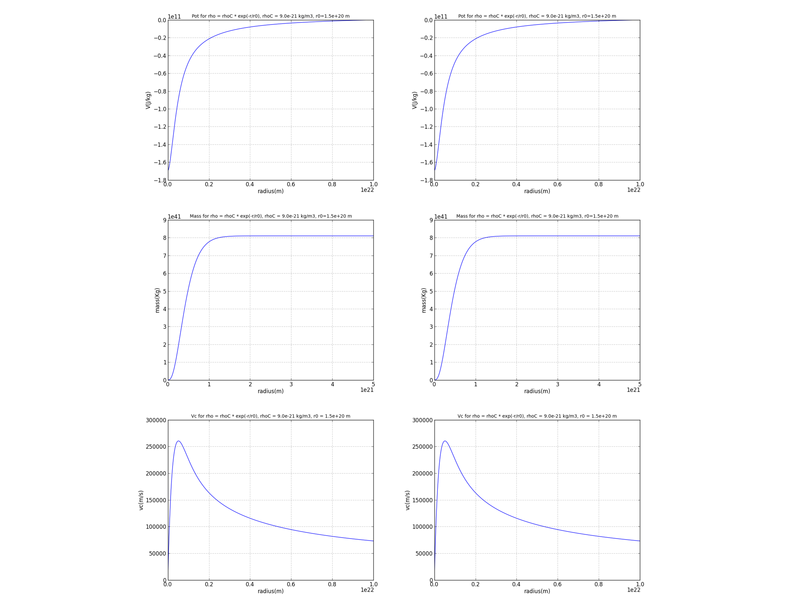
\includegraphics[scale=0.7]{allNumAn.png}
 \caption{\emph{izquierda: soluciones calculadas de forma numérica, derecha: analítica}}
\end{figure}

\end{description}

\clearpage

\section*{Variación de los parámetros ($r_0$ y $\rho_c$)}

\begin{description}
\item Los gráficos se realizaron con un programa python (exp\_compare.py) 
\item Se muestran los gráficos  para $\rho_c$ en $ \{2e-21,4e-21,9e-21,18e-21 \}  $ kg/m3 y $r_0$ en $\{1, 2, 5, 10 \} $ kpc. 
Todas las cantidades estan expresadas en las unidades SI: densidad kg/m3, distancia m, potencial J/kg, densidad proyectada kg/m2, vc m/s y se consideró la constante gravitacional $G = 6.6 * 10^{-11} m^3/(kg * s^2)$

\end{description}



\begin{figure}[!ht]
 \centering
 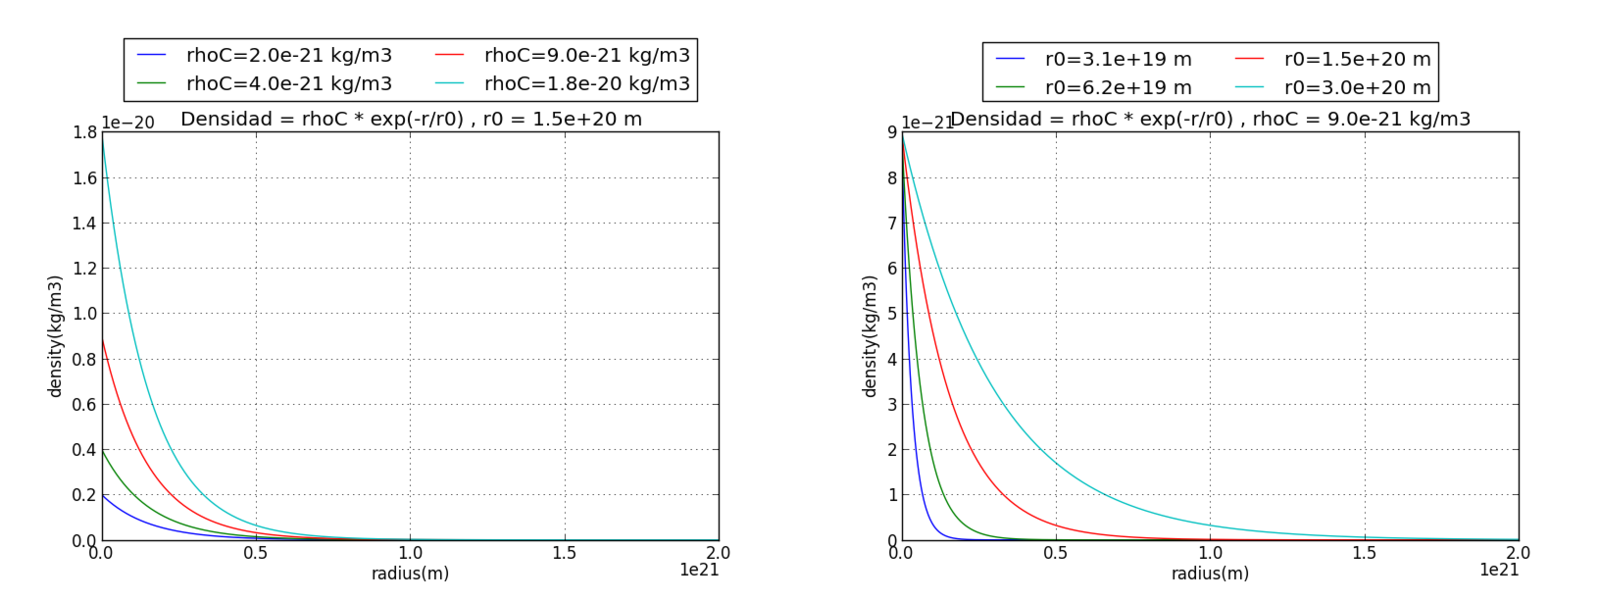
\includegraphics[scale=0.33]{densFinal.png}
 \caption{\emph{Densidad}}
\end{figure}


\begin{figure}[!ht]
 \centering
 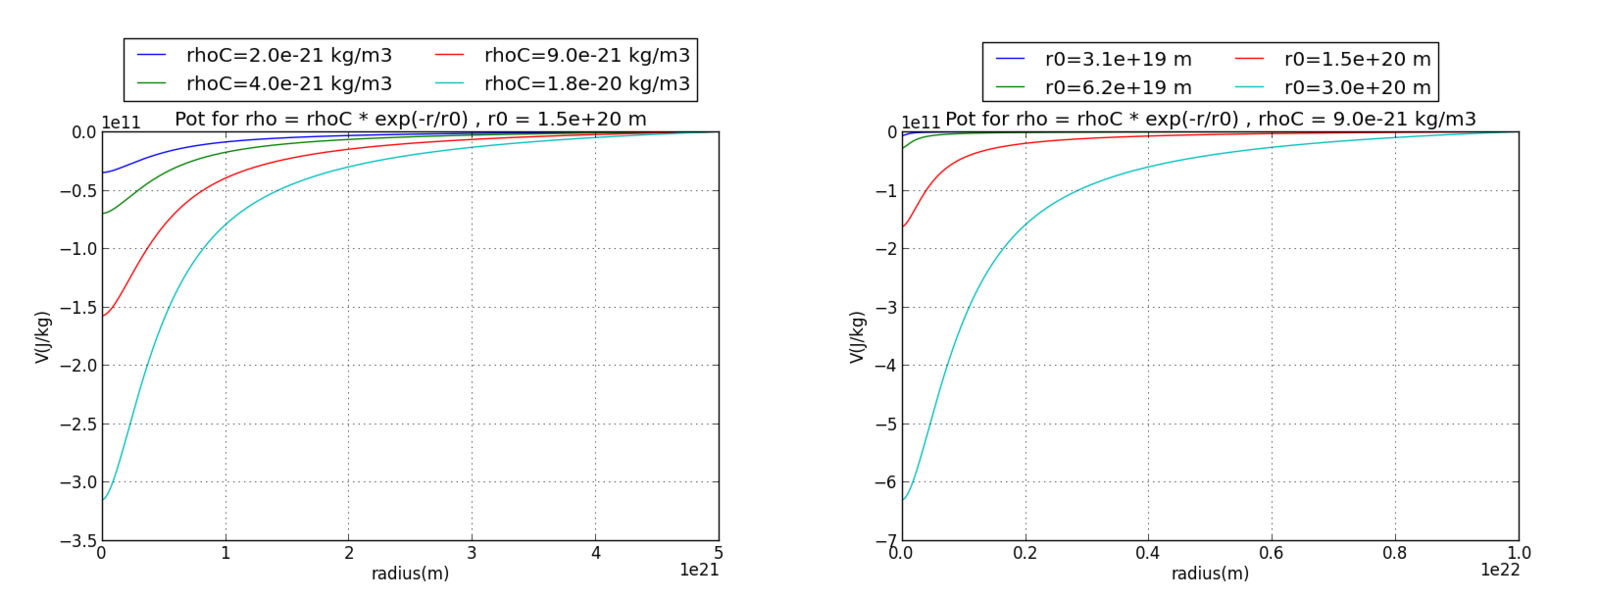
\includegraphics[scale=0.33]{potFinal.png}
 \caption{\emph{Potencial}}
\end{figure}


\begin{figure}[!ht]
 \centering
 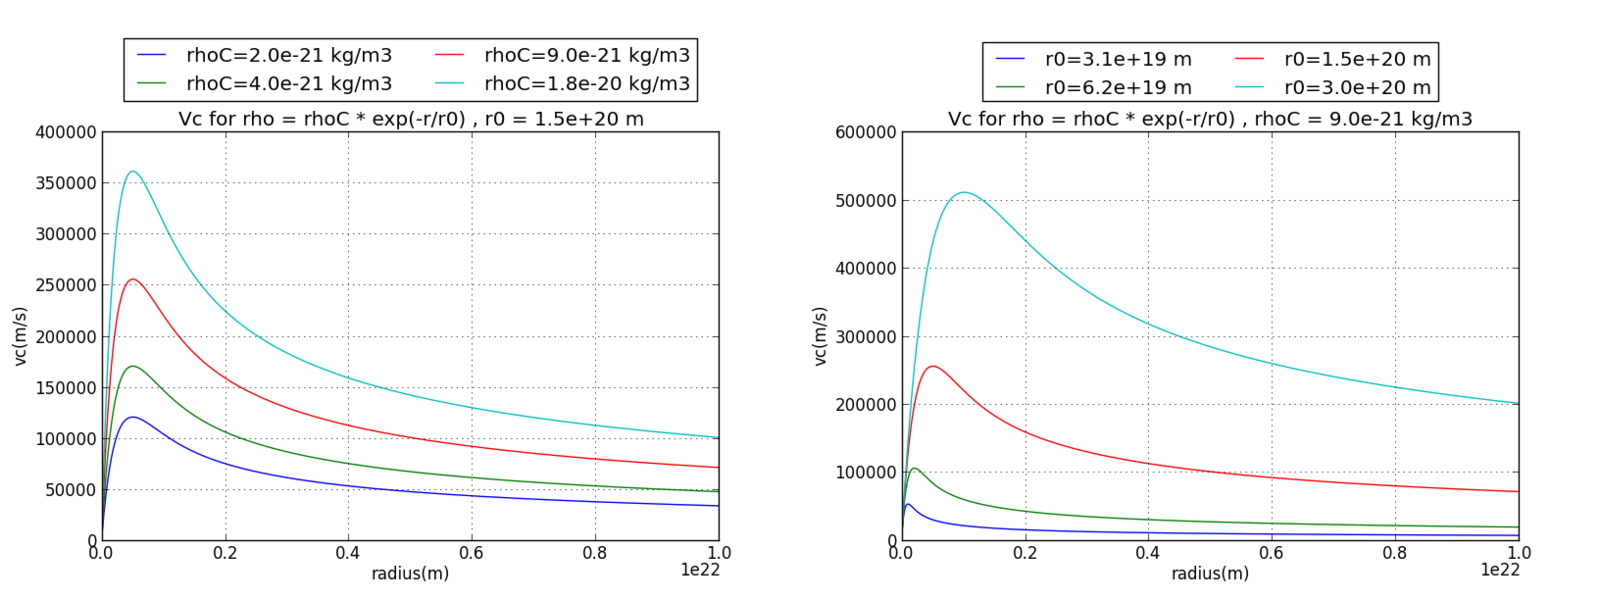
\includegraphics[scale=0.33]{vcFinal.png}
 \caption{\emph{Velocidad circular}}
\end{figure}


\begin{figure}[!ht]
 \centering
 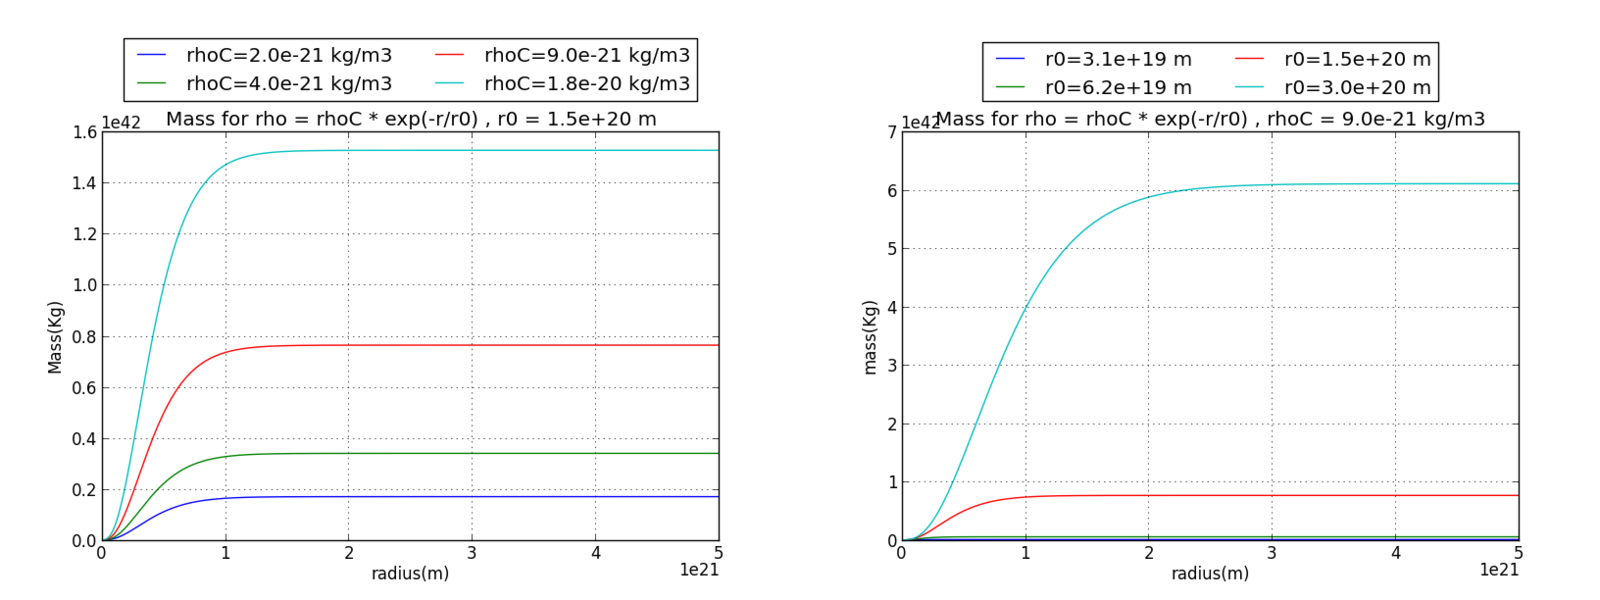
\includegraphics[scale=0.33]{massFinal.png}
 \caption{\emph{Masa}}
\end{figure}


\begin{figure}[!ht]
 \centering
 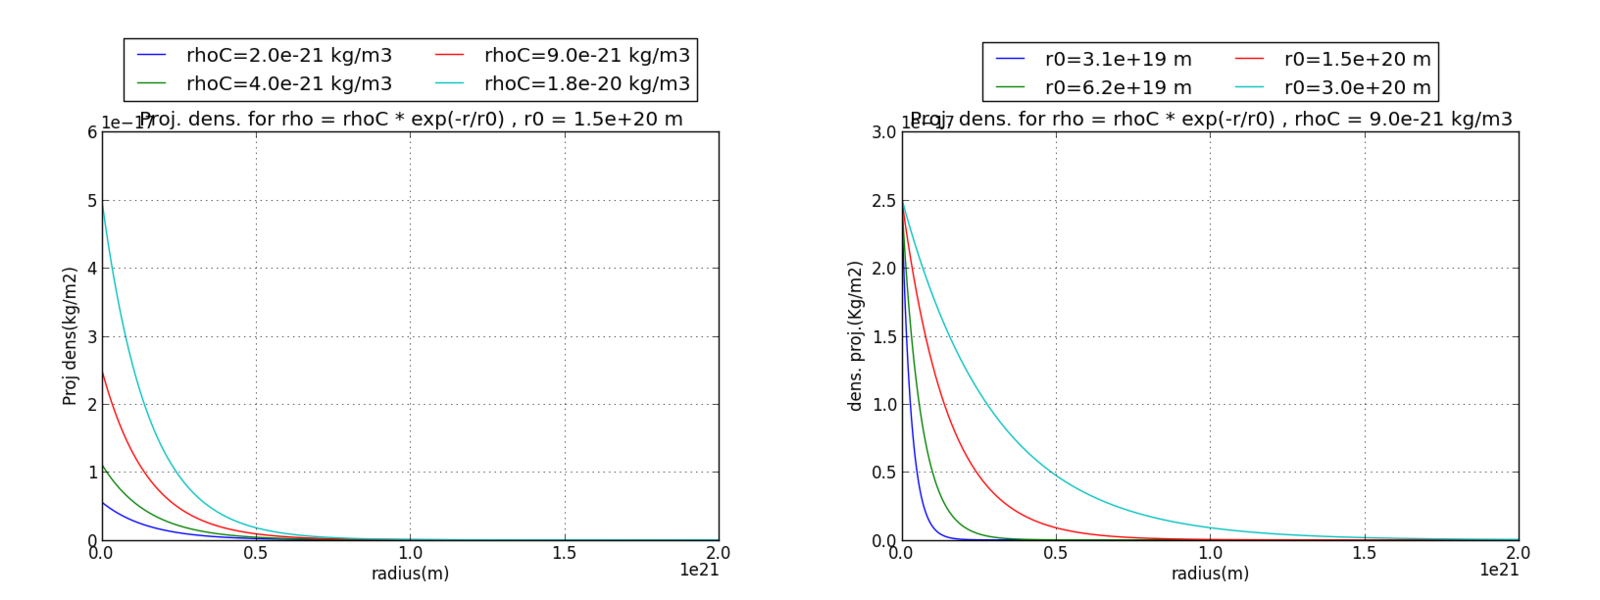
\includegraphics[scale=0.33]{dpFinal.png}
 \caption{\emph{Densidad proyectada}}
\end{figure}

\clearpage

\section*{Comparación con el potencial isócrono}


\subsection*{Solución analítica del potencial isocrono}

\begin{description}
\item Hay 2 parámetros configurables: b(b = 0 es equivalente a una masa puntual: toda la masa en el centro )  y M (la masa total del sistema) 
 
\item $ \Phi(r) =  -\frac{G  M}  {b + \sqrt{b^2 + r^2}}  $
\item usando sympy para hacer los cálculos (sympyPot.py) (las fórmulas salen como en el libro)
\item  Se define  $a = \sqrt{b^2 + r^2}$
\item $ \rho(r) =  M  ( \frac{3(b+a)a^2 - r^2(b+3a) }{4 \pi (b+a)^3  a^3 })$		
\item $ M(r) = M\frac{r^3}{(b + \sqrt{b^2 + r^2})^2 \sqrt{b^2 + r^2}} $ 
\item $ v_c(r) =  \sqrt{(G  M  r ^ 2)/((b + a)^2 * a)} $ 
\item La densidad proyectada se calcula como antes reemplazando la funcion de densidad
\end{description}



\subsection*{Comparación}
\begin{description}
\item Para comparar los gráficos de las funciones de 2 sistemas: uno con distribucion de densidad exponencial y otro con el modelo de potencial isócrono que tienen la misma densidad central y masa total:
\item Elegimos $r_0$ (el parametro de escala de la distribucion exponencial)= 5kpc (1.53e20) y $\rho_c$ = 9e-21 y ejecutamos el programa para dibujar la masa para la distribución exponencial. 
\item La masa total obtenida aqui y la misma $\rho_c$ metemos como parametros para calcular las funciones del potencial isocrono.
\item El parámetro b del potencial isócrono se calcula reemplazando r=0 en la fórmula de la densidad: $b = (\frac{3 M}{16 \pi \rho_c})^{\frac{1}{3}}$ 
  \end{description}

\begin{verbatim}
	python exp_plot.py --type=m --rmax=1e+22 --r0=1.53e20  --rhoC=9e-21
	python isochrone_plot.py --type=v --rmax=1e+22 --mass=8.1e+41  --rhoC=9e-21
\end{verbatim}

\begin{figure}[!ht]
 \centering
 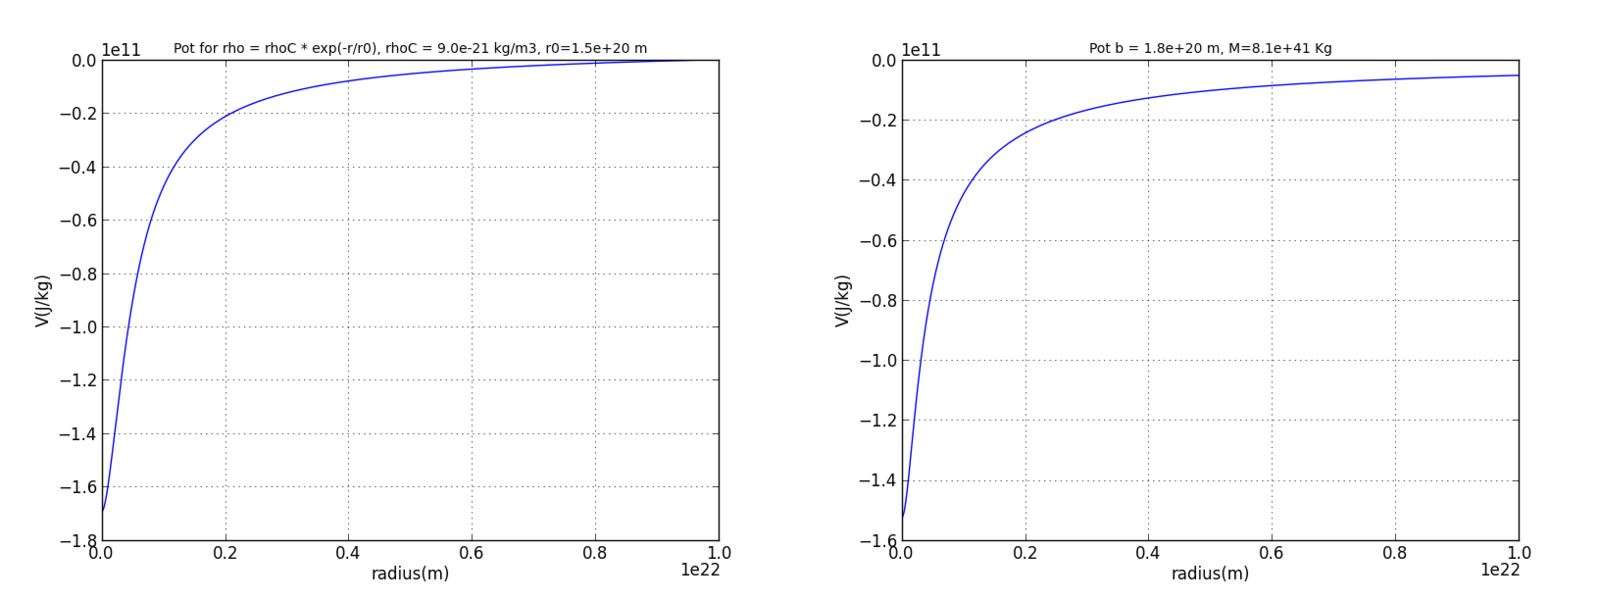
\includegraphics[scale=0.3]{potAnComp.png}
 \caption{\emph{Potencial comparado}}
\end{figure}

\begin{figure}[!ht]
 \centering
 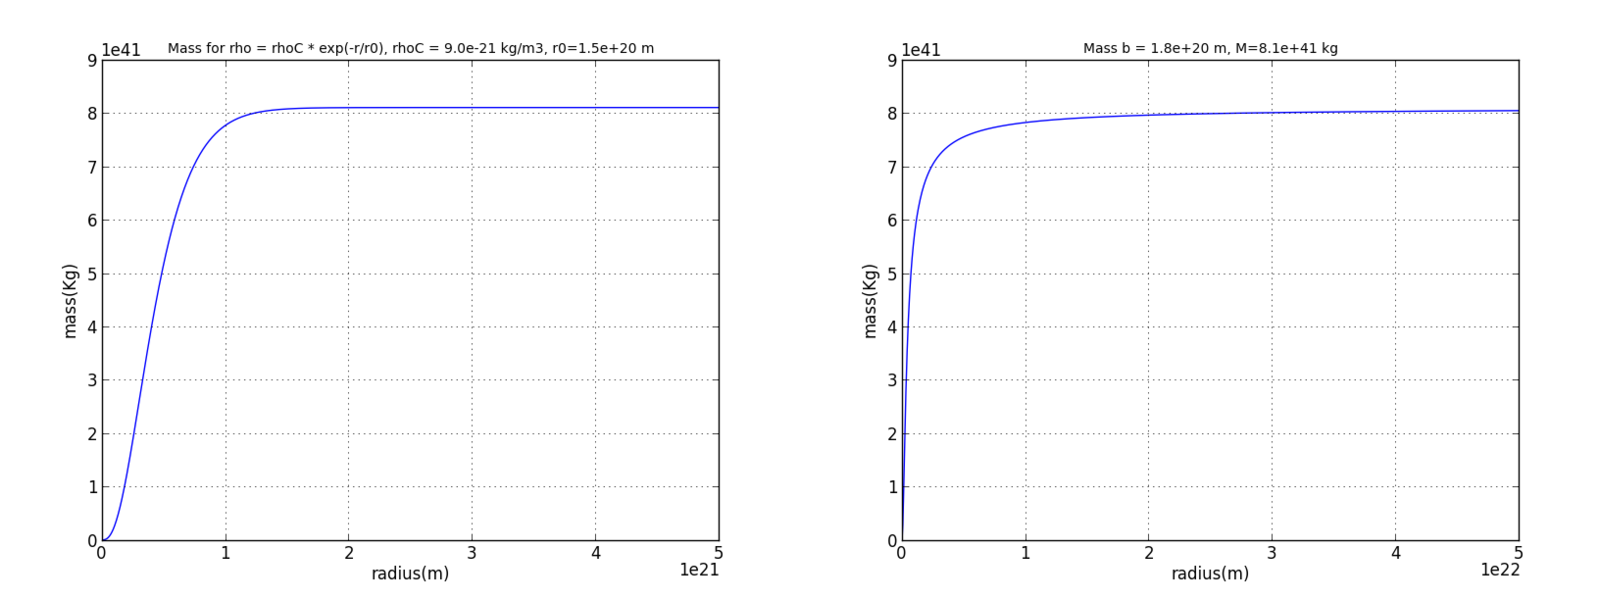
\includegraphics[scale=0.3]{massAnComp.png}
 \caption{\emph{Masa comparada}(Rmax en el caso del potencial isocrono = 10 * Rmax que en el caso de la distr. exp.)}
\end{figure}


\begin{figure}[!ht]
 \centering
 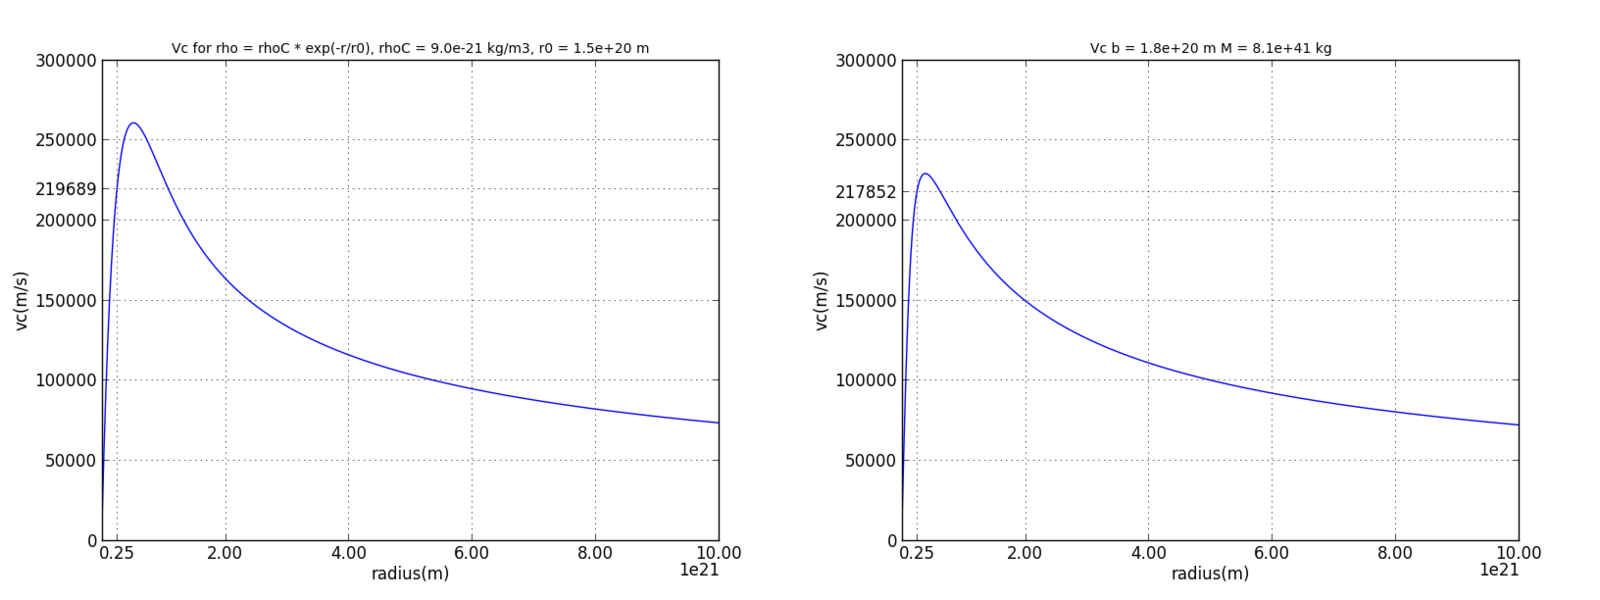
\includegraphics[scale=0.3]{vcAnComp.png}
 \caption{\emph{Velocidad comparada}}
\end{figure}

\begin{figure}[!ht]
 \centering
 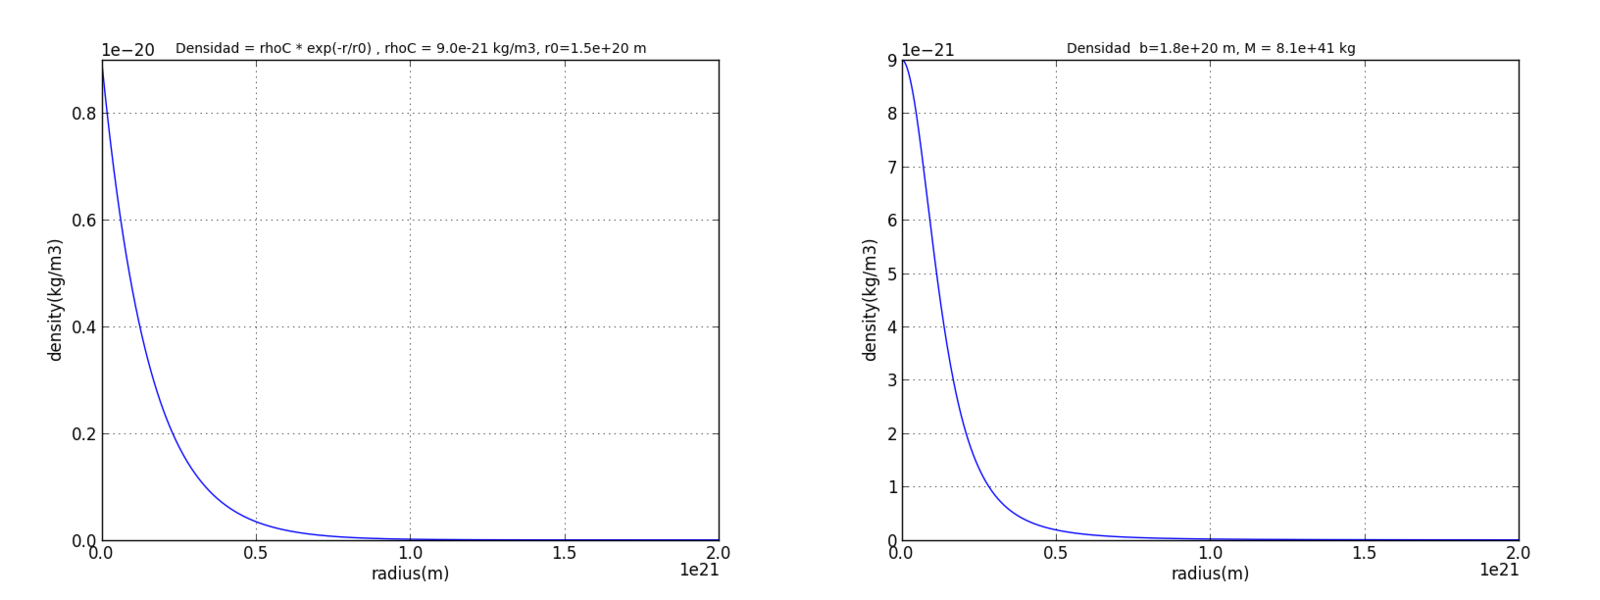
\includegraphics[scale=0.3]{densAnComp.png}
 \caption{\emph{Densidad comparada}}
\end{figure}

\begin{figure}[!ht]
 \centering
 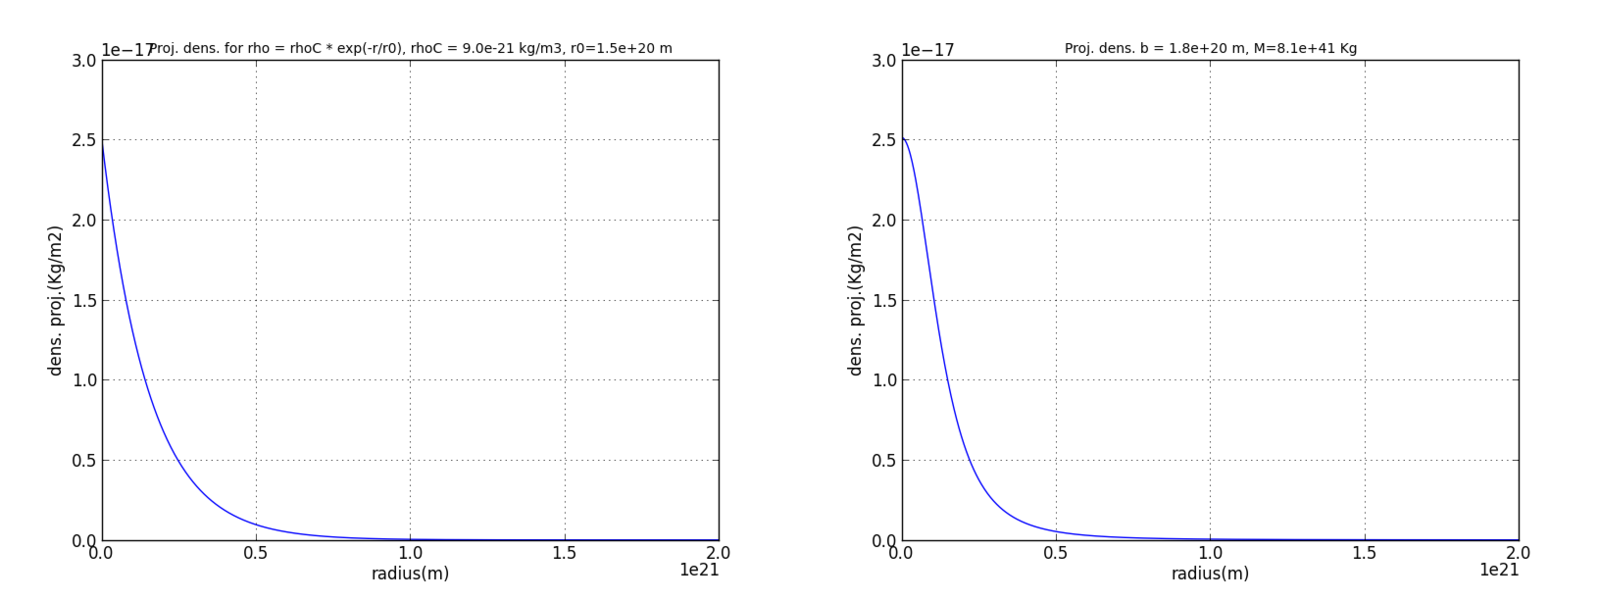
\includegraphics[scale=0.3]{dpAnComp.png}
 \caption{\emph{Densidad proyectada comparado}}
\end{figure}


\clearpage

\section*{Conclusiones}
\begin{description}
\item Para las 2 distribuciones cuando la densidad es casi 0 la masa encerrada en el radius correspondiente es casi toda la masa (despues de este radius la masa es casi constante), el potencial se acerca a 0 y vc tiene el máximo
\item Si la densidad decrece la densidad proyectada decrece más rápido visto que en el centro hay mas puntos para sumar la densidad (para integrar a lo largo de la linea de vision)

\item Para la distribución exponencial:

\begin{description}
	\item Variando el parámetro de escala $r_0$ (el radio en cual el logaritmo natural de la densidad decrece con una unidad comparado al logaritmo de la densidad central): si es mayor la densidad decrece mas lento (con respecto a la distancia del centro), la masa total  a va ser mayor igual que el máximo de la vc (pero van a crecer mas lento) y el potencial en el centro que va a decrecer mas despacio (igual que la densidad).	
\item Cuanto mayor es la densidad central, mayor será la masa, la vc  y el potencial en el centro igual que en el caso de aumentar el valor del parametro de escala $r_0$ pero la diferencia es menor que en el caso de variar $r_0$
\end{description}

\item En el caso del potencial isocrono la densidad tiene una porción muy pequeña en el centro casi constante, pero despues decrece mas rapido que en el caso de la distribucion exponencial, lo que hace que la masa crece mucho mas despacio(y la masa total es la misma)  y el potencial en el centro va a ser menor, igual que la vc máxima.
\item Observamos que en los 2 casos la  velocidad circular al radio donde se encuentra el sol es alrededor de 2.2e5 m/s, pero la masa total es menor de 2e42 (8.1e+41, 2.4 veces menor, porque?)
\end{description}


\clearpage

\section*{Código}

\begin{itemize}

\item Los programas python, imagenes, pdf e incluso el tex están en el repositorio git: 
	\url{https://github.com/beevageeva/potencial} 
Allí está la descripción y ejemplos de uso.

	 
\item Por razones históricas hay otro programa python mas general  (pt.py)  
\item Se muestran los gráficos en el caso A = B = 1 ($\implies r_0= \rho_c =1$) y constantes de integración 0, el segundo gráfico está calculado con la solución analítica: ver calc\_exp.py)

\begin{verbatim}
python pt.py --type=p --test=calc_exp --k=0,-8e-10 
python pt.py --type=v --test=calc_exp 
python pt.py --type=m --test=calc_exp 

\end{verbatim}
\begin{figure}[!ht]
 \centering
 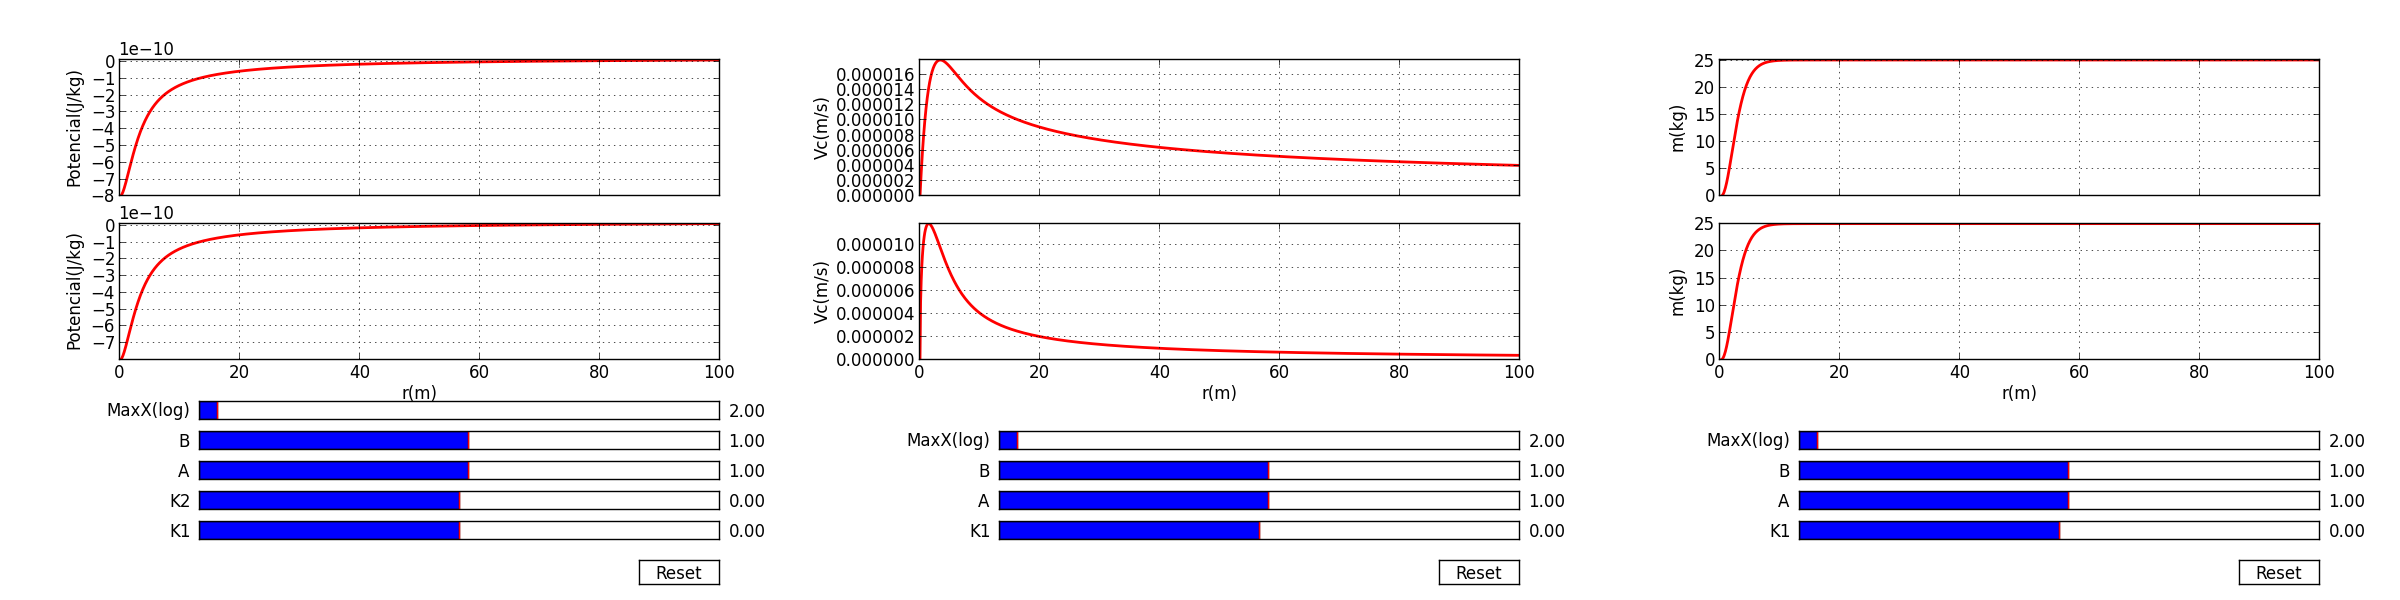
\includegraphics[scale=0.18]{ptAll.png}
 \caption{\emph{Salidas de las ejecuciones de pt.py de arriba}}
\end{figure}



\end{itemize}





\end{document}

